\documentclass{article}
\usepackage{tikz}
\usetikzlibrary{patterns}
\usepackage{subcaption}
\usepackage[margin=1in]{geometry}

\begin{document}

\begin{figure}[ht]
    \centering
    \begin{subfigure}{0.45\textwidth}
        \centering
        \resizebox{\textwidth}{!}{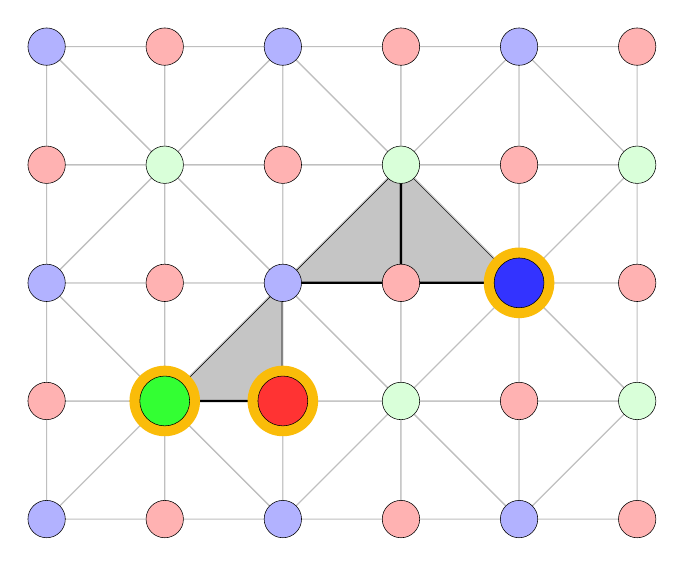
\begin{tikzpicture}[scale=1.5]
    \filldraw[fill=white, draw=gray!50, , fill opacity=1.0] (-2,-2) -- (-1,-2) -- (-1,-1) -- cycle;
    \filldraw[fill=white, draw=gray!50, , fill opacity=1.0] (-2,-2) -- (-2,-1) -- (-1,-1) -- cycle;
    \filldraw[fill=white, draw=gray!50, , fill opacity=1.0] (-2,0) -- (-2,-1) -- (-1,-1) -- cycle;
    \filldraw[fill=white, draw=gray!50, , fill opacity=1.0] (-2,0) -- (-1,0) -- (-1,-1) -- cycle;
    \filldraw[fill=white, draw=gray!50, , fill opacity=1.0] (-2,0) -- (-1,0) -- (-1,1) -- cycle;
    \filldraw[fill=white, draw=gray!50, , fill opacity=1.0] (-2,0) -- (-2,1) -- (-1,1) -- cycle;
    \filldraw[fill=white, draw=gray!50, , fill opacity=1.0] (-2,2) -- (-2,1) -- (-1,1) -- cycle;
    \filldraw[fill=white, draw=gray!50, , fill opacity=1.0] (-2,2) -- (-1,2) -- (-1,1) -- cycle;
    \filldraw[fill=white, draw=gray!50, , fill opacity=1.0] (0,-2) -- (-1,-2) -- (-1,-1) -- cycle;
    \filldraw[fill=white, draw=gray!50, , fill opacity=1.0] (0,-2) -- (0,-1) -- (-1,-1) -- cycle;
    \filldraw[fill=gray!50, draw=black, thick, fill opacity=0.9] (0,0) -- (0,-1) -- (-1,-1) -- cycle;
    \filldraw[fill=white, draw=gray!50, , fill opacity=1.0] (0,0) -- (-1,0) -- (-1,-1) -- cycle;
    \filldraw[fill=white, draw=gray!50, , fill opacity=1.0] (0,0) -- (-1,0) -- (-1,1) -- cycle;
    \filldraw[fill=white, draw=gray!50, , fill opacity=1.0] (0,0) -- (0,1) -- (-1,1) -- cycle;
    \filldraw[fill=white, draw=gray!50, , fill opacity=1.0] (0,2) -- (0,1) -- (-1,1) -- cycle;
    \filldraw[fill=white, draw=gray!50, , fill opacity=1.0] (0,2) -- (-1,2) -- (-1,1) -- cycle;
    \filldraw[fill=white, draw=gray!50, , fill opacity=1.0] (0,-2) -- (1,-2) -- (1,-1) -- cycle;
    \filldraw[fill=white, draw=gray!50, , fill opacity=1.0] (0,-2) -- (0,-1) -- (1,-1) -- cycle;
    \filldraw[fill=white, draw=gray!50, , fill opacity=1.0] (0,0) -- (0,-1) -- (1,-1) -- cycle;
    \filldraw[fill=white, draw=gray!50, , fill opacity=1.0] (0,0) -- (1,0) -- (1,-1) -- cycle;
    \filldraw[fill=gray!50, draw=black, thick, fill opacity=0.9] (0,0) -- (1,0) -- (1,1) -- cycle;
    \filldraw[fill=white, draw=gray!50, , fill opacity=1.0] (0,0) -- (0,1) -- (1,1) -- cycle;
    \filldraw[fill=white, draw=gray!50, , fill opacity=1.0] (0,2) -- (0,1) -- (1,1) -- cycle;
    \filldraw[fill=white, draw=gray!50, , fill opacity=1.0] (0,2) -- (1,2) -- (1,1) -- cycle;
    \filldraw[fill=white, draw=gray!50, , fill opacity=1.0] (2,-2) -- (1,-2) -- (1,-1) -- cycle;
    \filldraw[fill=white, draw=gray!50, , fill opacity=1.0] (2,-2) -- (2,-1) -- (1,-1) -- cycle;
    \filldraw[fill=white, draw=gray!50, , fill opacity=1.0] (2,0) -- (2,-1) -- (1,-1) -- cycle;
    \filldraw[fill=white, draw=gray!50, , fill opacity=1.0] (2,0) -- (1,0) -- (1,-1) -- cycle;
    \filldraw[fill=gray!50, draw=black, thick, fill opacity=0.9] (2,0) -- (1,0) -- (1,1) -- cycle;
    \filldraw[fill=white, draw=gray!50, , fill opacity=1.0] (2,0) -- (2,1) -- (1,1) -- cycle;
    \filldraw[fill=white, draw=gray!50, , fill opacity=1.0] (2,2) -- (2,1) -- (1,1) -- cycle;
    \filldraw[fill=white, draw=gray!50, , fill opacity=1.0] (2,2) -- (1,2) -- (1,1) -- cycle;
    \filldraw[fill=white, draw=gray!50, , fill opacity=1.0] (2,-2) -- (3,-2) -- (3,-1) -- cycle;
    \filldraw[fill=white, draw=gray!50, , fill opacity=1.0] (2,-2) -- (2,-1) -- (3,-1) -- cycle;
    \filldraw[fill=white, draw=gray!50, , fill opacity=1.0] (2,0) -- (2,-1) -- (3,-1) -- cycle;
    \filldraw[fill=white, draw=gray!50, , fill opacity=1.0] (2,0) -- (3,0) -- (3,-1) -- cycle;
    \filldraw[fill=white, draw=gray!50, , fill opacity=1.0] (2,0) -- (3,0) -- (3,1) -- cycle;
    \filldraw[fill=white, draw=gray!50, , fill opacity=1.0] (2,0) -- (2,1) -- (3,1) -- cycle;
    \filldraw[fill=white, draw=gray!50, , fill opacity=1.0] (2,2) -- (2,1) -- (3,1) -- cycle;
    \filldraw[fill=white, draw=gray!50, , fill opacity=1.0] (2,2) -- (3,2) -- (3,1) -- cycle;
    \filldraw[fill=blue!30, draw=black, very thin] (-2, -2) circle (4.5pt);
    \filldraw[fill=red!30, draw=black, very thin] (-2, -1) circle (4.5pt);
    \filldraw[fill=blue!30, draw=black, very thin] (-2, 0) circle (4.5pt);
    \filldraw[fill=red!30, draw=black, very thin] (-2, 1) circle (4.5pt);
    \filldraw[fill=blue!30, draw=black, very thin] (-2, 2) circle (4.5pt);
    \filldraw[fill=red!30, draw=black, very thin] (-1, -2) circle (4.5pt);
    \filldraw[fill=yellow!50!orange, draw=none] (-1, -1) circle (8.5pt);
    \filldraw[fill=green!80, draw=black, very thin] (-1, -1) circle (6pt);
    \filldraw[fill=red!30, draw=black, very thin] (-1, 0) circle (4.5pt);
    \filldraw[fill=green!15, draw=black, very thin] (-1, 1) circle (4.5pt);
    \filldraw[fill=red!30, draw=black, very thin] (-1, 2) circle (4.5pt);
    \filldraw[fill=blue!30, draw=black, very thin] (0, -2) circle (4.5pt);
    \filldraw[fill=yellow!50!orange, draw=none] (0, -1) circle (8.5pt);
    \filldraw[fill=red!80, draw=black, very thin] (0, -1) circle (6pt);
    \filldraw[fill=blue!30, draw=black, very thin] (0, 0) circle (4.5pt);
    \filldraw[fill=red!30, draw=black, very thin] (0, 1) circle (4.5pt);
    \filldraw[fill=blue!30, draw=black, very thin] (0, 2) circle (4.5pt);
    \filldraw[fill=red!30, draw=black, very thin] (1, -2) circle (4.5pt);
    \filldraw[fill=green!15, draw=black, very thin] (1, -1) circle (4.5pt);
    \filldraw[fill=red!30, draw=black, very thin] (1, 0) circle (4.5pt);
    \filldraw[fill=green!15, draw=black, very thin] (1, 1) circle (4.5pt);
    \filldraw[fill=red!30, draw=black, very thin] (1, 2) circle (4.5pt);
    \filldraw[fill=blue!30, draw=black, very thin] (2, -2) circle (4.5pt);
    \filldraw[fill=red!30, draw=black, very thin] (2, -1) circle (4.5pt);
    \filldraw[fill=yellow!50!orange, draw=none] (2, 0) circle (8.5pt);
    \filldraw[fill=blue!80, draw=black, very thin] (2, 0) circle (6pt);
    \filldraw[fill=red!30, draw=black, very thin] (2, 1) circle (4.5pt);
    \filldraw[fill=blue!30, draw=black, very thin] (2, 2) circle (4.5pt);
    \filldraw[fill=red!30, draw=black, very thin] (3, -2) circle (4.5pt);
    \filldraw[fill=green!15, draw=black, very thin] (3, -1) circle (4.5pt);
    \filldraw[fill=red!30, draw=black, very thin] (3, 0) circle (4.5pt);
    \filldraw[fill=green!15, draw=black, very thin] (3, 1) circle (4.5pt);
    \filldraw[fill=red!30, draw=black, very thin] (3, 2) circle (4.5pt);
\end{tikzpicture}
}
        \caption{Full Lattice (Errors in gray)}
    \end{subfigure}
    \hfill
    \begin{subfigure}{0.45\textwidth}
        \centering
        \resizebox{\textwidth}{!}{\input{non_boundary_ok_b.tex}}
        \caption{$\mathcal{L}_{RG}$ (MWPM matches correctly)}
    \end{subfigure}
    
    \vspace{1cm}
    
    \begin{subfigure}{0.45\textwidth}
        \centering
        \resizebox{\textwidth}{!}{\input{non_boundary_ok_c.tex}}
        \caption{$\mathcal{L}_{RB}$ (MWPM matches correctly)}
    \end{subfigure}
    \hfill
    \begin{subfigure}{0.45\textwidth}
        \centering
        \resizebox{\textwidth}{!}{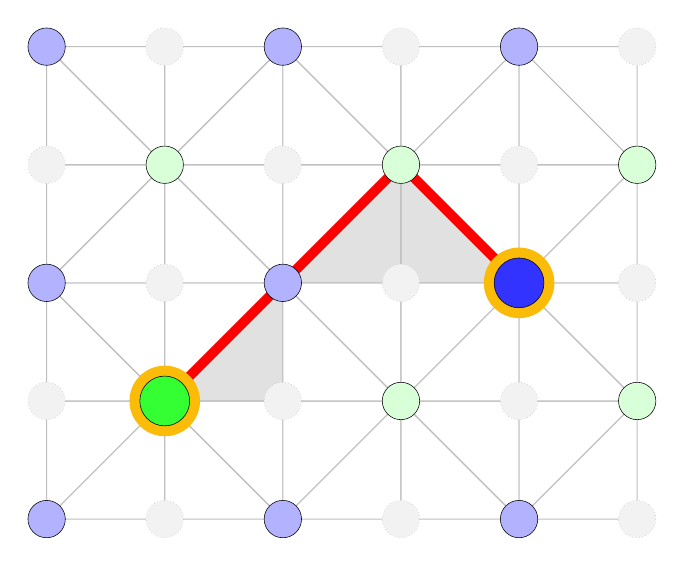
\begin{tikzpicture}[scale=1.5]
    \filldraw[fill=white, draw=gray!50, , fill opacity=1.0] (-2,-2) -- (-1,-2) -- (-1,-1) -- cycle;
    \filldraw[fill=white, draw=gray!50, , fill opacity=1.0] (-2,-2) -- (-2,-1) -- (-1,-1) -- cycle;
    \filldraw[fill=white, draw=gray!50, , fill opacity=1.0] (-2,0) -- (-2,-1) -- (-1,-1) -- cycle;
    \filldraw[fill=white, draw=gray!50, , fill opacity=1.0] (-2,0) -- (-1,0) -- (-1,-1) -- cycle;
    \filldraw[fill=white, draw=gray!50, , fill opacity=1.0] (-2,0) -- (-1,0) -- (-1,1) -- cycle;
    \filldraw[fill=white, draw=gray!50, , fill opacity=1.0] (-2,0) -- (-2,1) -- (-1,1) -- cycle;
    \filldraw[fill=white, draw=gray!50, , fill opacity=1.0] (-2,2) -- (-2,1) -- (-1,1) -- cycle;
    \filldraw[fill=white, draw=gray!50, , fill opacity=1.0] (-2,2) -- (-1,2) -- (-1,1) -- cycle;
    \filldraw[fill=white, draw=gray!50, , fill opacity=1.0] (0,-2) -- (-1,-2) -- (-1,-1) -- cycle;
    \filldraw[fill=white, draw=gray!50, , fill opacity=1.0] (0,-2) -- (0,-1) -- (-1,-1) -- cycle;
    \filldraw[fill=gray!30, draw=gray!50, , fill opacity=0.8] (0,0) -- (0,-1) -- (-1,-1) -- cycle;
    \filldraw[fill=white, draw=gray!50, , fill opacity=1.0] (0,0) -- (-1,0) -- (-1,-1) -- cycle;
    \filldraw[fill=white, draw=gray!50, , fill opacity=1.0] (0,0) -- (-1,0) -- (-1,1) -- cycle;
    \filldraw[fill=white, draw=gray!50, , fill opacity=1.0] (0,0) -- (0,1) -- (-1,1) -- cycle;
    \filldraw[fill=white, draw=gray!50, , fill opacity=1.0] (0,2) -- (0,1) -- (-1,1) -- cycle;
    \filldraw[fill=white, draw=gray!50, , fill opacity=1.0] (0,2) -- (-1,2) -- (-1,1) -- cycle;
    \filldraw[fill=white, draw=gray!50, , fill opacity=1.0] (0,-2) -- (1,-2) -- (1,-1) -- cycle;
    \filldraw[fill=white, draw=gray!50, , fill opacity=1.0] (0,-2) -- (0,-1) -- (1,-1) -- cycle;
    \filldraw[fill=white, draw=gray!50, , fill opacity=1.0] (0,0) -- (0,-1) -- (1,-1) -- cycle;
    \filldraw[fill=white, draw=gray!50, , fill opacity=1.0] (0,0) -- (1,0) -- (1,-1) -- cycle;
    \filldraw[fill=gray!30, draw=gray!50, , fill opacity=0.8] (0,0) -- (1,0) -- (1,1) -- cycle;
    \filldraw[fill=white, draw=gray!50, , fill opacity=1.0] (0,0) -- (0,1) -- (1,1) -- cycle;
    \filldraw[fill=white, draw=gray!50, , fill opacity=1.0] (0,2) -- (0,1) -- (1,1) -- cycle;
    \filldraw[fill=white, draw=gray!50, , fill opacity=1.0] (0,2) -- (1,2) -- (1,1) -- cycle;
    \filldraw[fill=white, draw=gray!50, , fill opacity=1.0] (2,-2) -- (1,-2) -- (1,-1) -- cycle;
    \filldraw[fill=white, draw=gray!50, , fill opacity=1.0] (2,-2) -- (2,-1) -- (1,-1) -- cycle;
    \filldraw[fill=white, draw=gray!50, , fill opacity=1.0] (2,0) -- (2,-1) -- (1,-1) -- cycle;
    \filldraw[fill=white, draw=gray!50, , fill opacity=1.0] (2,0) -- (1,0) -- (1,-1) -- cycle;
    \filldraw[fill=gray!30, draw=gray!50, , fill opacity=0.8] (2,0) -- (1,0) -- (1,1) -- cycle;
    \filldraw[fill=white, draw=gray!50, , fill opacity=1.0] (2,0) -- (2,1) -- (1,1) -- cycle;
    \filldraw[fill=white, draw=gray!50, , fill opacity=1.0] (2,2) -- (2,1) -- (1,1) -- cycle;
    \filldraw[fill=white, draw=gray!50, , fill opacity=1.0] (2,2) -- (1,2) -- (1,1) -- cycle;
    \filldraw[fill=white, draw=gray!50, , fill opacity=1.0] (2,-2) -- (3,-2) -- (3,-1) -- cycle;
    \filldraw[fill=white, draw=gray!50, , fill opacity=1.0] (2,-2) -- (2,-1) -- (3,-1) -- cycle;
    \filldraw[fill=white, draw=gray!50, , fill opacity=1.0] (2,0) -- (2,-1) -- (3,-1) -- cycle;
    \filldraw[fill=white, draw=gray!50, , fill opacity=1.0] (2,0) -- (3,0) -- (3,-1) -- cycle;
    \filldraw[fill=white, draw=gray!50, , fill opacity=1.0] (2,0) -- (3,0) -- (3,1) -- cycle;
    \filldraw[fill=white, draw=gray!50, , fill opacity=1.0] (2,0) -- (2,1) -- (3,1) -- cycle;
    \filldraw[fill=white, draw=gray!50, , fill opacity=1.0] (2,2) -- (2,1) -- (3,1) -- cycle;
    \filldraw[fill=white, draw=gray!50, , fill opacity=1.0] (2,2) -- (3,2) -- (3,1) -- cycle;
    \draw[red, line width=3.5pt] (-1,-1) -- (0,0) -- (1,1) -- (2,0);
    \filldraw[fill=blue!30, draw=black, very thin] (-2, -2) circle (4.5pt);
    \filldraw[fill=gray!10, draw=gray!50, densely dotted, very thin] (-2, -1) circle (4.5pt);
    \filldraw[fill=blue!30, draw=black, very thin] (-2, 0) circle (4.5pt);
    \filldraw[fill=gray!10, draw=gray!50, densely dotted, very thin] (-2, 1) circle (4.5pt);
    \filldraw[fill=blue!30, draw=black, very thin] (-2, 2) circle (4.5pt);
    \filldraw[fill=gray!10, draw=gray!50, densely dotted, very thin] (-1, -2) circle (4.5pt);
    \filldraw[fill=yellow!50!orange, draw=none] (-1, -1) circle (8.5pt);
    \filldraw[fill=green!80, draw=black, very thin] (-1, -1) circle (6pt);
    \filldraw[fill=gray!10, draw=gray!50, densely dotted, very thin] (-1, 0) circle (4.5pt);
    \filldraw[fill=green!15, draw=black, very thin] (-1, 1) circle (4.5pt);
    \filldraw[fill=gray!10, draw=gray!50, densely dotted, very thin] (-1, 2) circle (4.5pt);
    \filldraw[fill=blue!30, draw=black, very thin] (0, -2) circle (4.5pt);
    \filldraw[fill=gray!10, draw=gray!50, densely dotted, very thin] (0, -1) circle (4.5pt);
    \filldraw[fill=blue!30, draw=black, very thin] (0, 0) circle (4.5pt);
    \filldraw[fill=gray!10, draw=gray!50, densely dotted, very thin] (0, 1) circle (4.5pt);
    \filldraw[fill=blue!30, draw=black, very thin] (0, 2) circle (4.5pt);
    \filldraw[fill=gray!10, draw=gray!50, densely dotted, very thin] (1, -2) circle (4.5pt);
    \filldraw[fill=green!15, draw=black, very thin] (1, -1) circle (4.5pt);
    \filldraw[fill=gray!10, draw=gray!50, densely dotted, very thin] (1, 0) circle (4.5pt);
    \filldraw[fill=green!15, draw=black, very thin] (1, 1) circle (4.5pt);
    \filldraw[fill=gray!10, draw=gray!50, densely dotted, very thin] (1, 2) circle (4.5pt);
    \filldraw[fill=blue!30, draw=black, very thin] (2, -2) circle (4.5pt);
    \filldraw[fill=gray!10, draw=gray!50, densely dotted, very thin] (2, -1) circle (4.5pt);
    \filldraw[fill=yellow!50!orange, draw=none] (2, 0) circle (8.5pt);
    \filldraw[fill=blue!80, draw=black, very thin] (2, 0) circle (6pt);
    \filldraw[fill=gray!10, draw=gray!50, densely dotted, very thin] (2, 1) circle (4.5pt);
    \filldraw[fill=blue!30, draw=black, very thin] (2, 2) circle (4.5pt);
    \filldraw[fill=gray!10, draw=gray!50, densely dotted, very thin] (3, -2) circle (4.5pt);
    \filldraw[fill=green!15, draw=black, very thin] (3, -1) circle (4.5pt);
    \filldraw[fill=gray!10, draw=gray!50, densely dotted, very thin] (3, 0) circle (4.5pt);
    \filldraw[fill=green!15, draw=black, very thin] (3, 1) circle (4.5pt);
    \filldraw[fill=gray!10, draw=gray!50, densely dotted, very thin] (3, 2) circle (4.5pt);
\end{tikzpicture}
}
        \caption{$\mathcal{L}_{GB}$ (MWPM matches correctly)}
    \end{subfigure}
    \vspace{1cm}
    
    \begin{subfigure}{0.45\textwidth}
        \centering
        \resizebox{\textwidth}{!}{\input{non_boundary_ok_e.tex}}
        \caption{Projection Decoder (Successful Correction)}
    \end{subfigure}
    \hfill
    \begin{subfigure}{0.45\textwidth}
        \centering
        \resizebox{\textwidth}{!}{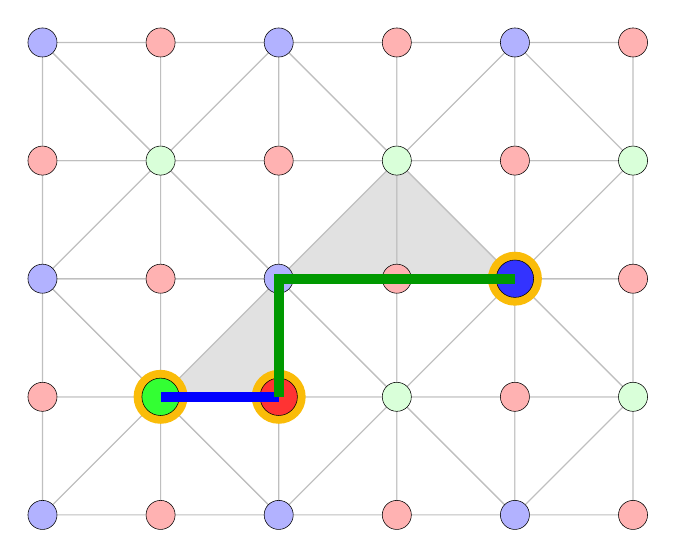
\begin{tikzpicture}[scale=1.5]
    \filldraw[fill=white, draw=gray!50, , fill opacity=1.0] (-2,-2) -- (-1,-2) -- (-1,-1) -- cycle;
    \filldraw[fill=white, draw=gray!50, , fill opacity=1.0] (-2,-2) -- (-2,-1) -- (-1,-1) -- cycle;
    \filldraw[fill=white, draw=gray!50, , fill opacity=1.0] (-2,0) -- (-2,-1) -- (-1,-1) -- cycle;
    \filldraw[fill=white, draw=gray!50, , fill opacity=1.0] (-2,0) -- (-1,0) -- (-1,-1) -- cycle;
    \filldraw[fill=white, draw=gray!50, , fill opacity=1.0] (-2,0) -- (-1,0) -- (-1,1) -- cycle;
    \filldraw[fill=white, draw=gray!50, , fill opacity=1.0] (-2,0) -- (-2,1) -- (-1,1) -- cycle;
    \filldraw[fill=white, draw=gray!50, , fill opacity=1.0] (-2,2) -- (-2,1) -- (-1,1) -- cycle;
    \filldraw[fill=white, draw=gray!50, , fill opacity=1.0] (-2,2) -- (-1,2) -- (-1,1) -- cycle;
    \filldraw[fill=white, draw=gray!50, , fill opacity=1.0] (0,-2) -- (-1,-2) -- (-1,-1) -- cycle;
    \filldraw[fill=white, draw=gray!50, , fill opacity=1.0] (0,-2) -- (0,-1) -- (-1,-1) -- cycle;
    \filldraw[fill=gray!30, draw=gray!50, , fill opacity=0.8] (0,0) -- (0,-1) -- (-1,-1) -- cycle;
    \filldraw[fill=white, draw=gray!50, , fill opacity=1.0] (0,0) -- (-1,0) -- (-1,-1) -- cycle;
    \filldraw[fill=white, draw=gray!50, , fill opacity=1.0] (0,0) -- (-1,0) -- (-1,1) -- cycle;
    \filldraw[fill=white, draw=gray!50, , fill opacity=1.0] (0,0) -- (0,1) -- (-1,1) -- cycle;
    \filldraw[fill=white, draw=gray!50, , fill opacity=1.0] (0,2) -- (0,1) -- (-1,1) -- cycle;
    \filldraw[fill=white, draw=gray!50, , fill opacity=1.0] (0,2) -- (-1,2) -- (-1,1) -- cycle;
    \filldraw[fill=white, draw=gray!50, , fill opacity=1.0] (0,-2) -- (1,-2) -- (1,-1) -- cycle;
    \filldraw[fill=white, draw=gray!50, , fill opacity=1.0] (0,-2) -- (0,-1) -- (1,-1) -- cycle;
    \filldraw[fill=white, draw=gray!50, , fill opacity=1.0] (0,0) -- (0,-1) -- (1,-1) -- cycle;
    \filldraw[fill=white, draw=gray!50, , fill opacity=1.0] (0,0) -- (1,0) -- (1,-1) -- cycle;
    \filldraw[fill=gray!30, draw=gray!50, , fill opacity=0.8] (0,0) -- (1,0) -- (1,1) -- cycle;
    \filldraw[fill=white, draw=gray!50, , fill opacity=1.0] (0,0) -- (0,1) -- (1,1) -- cycle;
    \filldraw[fill=white, draw=gray!50, , fill opacity=1.0] (0,2) -- (0,1) -- (1,1) -- cycle;
    \filldraw[fill=white, draw=gray!50, , fill opacity=1.0] (0,2) -- (1,2) -- (1,1) -- cycle;
    \filldraw[fill=white, draw=gray!50, , fill opacity=1.0] (2,-2) -- (1,-2) -- (1,-1) -- cycle;
    \filldraw[fill=white, draw=gray!50, , fill opacity=1.0] (2,-2) -- (2,-1) -- (1,-1) -- cycle;
    \filldraw[fill=white, draw=gray!50, , fill opacity=1.0] (2,0) -- (2,-1) -- (1,-1) -- cycle;
    \filldraw[fill=white, draw=gray!50, , fill opacity=1.0] (2,0) -- (1,0) -- (1,-1) -- cycle;
    \filldraw[fill=gray!30, draw=gray!50, , fill opacity=0.8] (2,0) -- (1,0) -- (1,1) -- cycle;
    \filldraw[fill=white, draw=gray!50, , fill opacity=1.0] (2,0) -- (2,1) -- (1,1) -- cycle;
    \filldraw[fill=white, draw=gray!50, , fill opacity=1.0] (2,2) -- (2,1) -- (1,1) -- cycle;
    \filldraw[fill=white, draw=gray!50, , fill opacity=1.0] (2,2) -- (1,2) -- (1,1) -- cycle;
    \filldraw[fill=white, draw=gray!50, , fill opacity=1.0] (2,-2) -- (3,-2) -- (3,-1) -- cycle;
    \filldraw[fill=white, draw=gray!50, , fill opacity=1.0] (2,-2) -- (2,-1) -- (3,-1) -- cycle;
    \filldraw[fill=white, draw=gray!50, , fill opacity=1.0] (2,0) -- (2,-1) -- (3,-1) -- cycle;
    \filldraw[fill=white, draw=gray!50, , fill opacity=1.0] (2,0) -- (3,0) -- (3,-1) -- cycle;
    \filldraw[fill=white, draw=gray!50, , fill opacity=1.0] (2,0) -- (3,0) -- (3,1) -- cycle;
    \filldraw[fill=white, draw=gray!50, , fill opacity=1.0] (2,0) -- (2,1) -- (3,1) -- cycle;
    \filldraw[fill=white, draw=gray!50, , fill opacity=1.0] (2,2) -- (2,1) -- (3,1) -- cycle;
    \filldraw[fill=white, draw=gray!50, , fill opacity=1.0] (2,2) -- (3,2) -- (3,1) -- cycle;
    \filldraw[fill=blue!30, draw=black, very thin] (-2, -2) circle (3.5pt);
    \filldraw[fill=red!30, draw=black, very thin] (-2, -1) circle (3.5pt);
    \filldraw[fill=blue!30, draw=black, very thin] (-2, 0) circle (3.5pt);
    \filldraw[fill=red!30, draw=black, very thin] (-2, 1) circle (3.5pt);
    \filldraw[fill=blue!30, draw=black, very thin] (-2, 2) circle (3.5pt);
    \filldraw[fill=red!30, draw=black, very thin] (-1, -2) circle (3.5pt);
    \filldraw[fill=yellow!50!orange, draw=none] (-1, -1) circle (6.5pt);
    \filldraw[fill=green!80, draw=black, very thin] (-1, -1) circle (4.5pt);
    \filldraw[fill=red!30, draw=black, very thin] (-1, 0) circle (3.5pt);
    \filldraw[fill=green!15, draw=black, very thin] (-1, 1) circle (3.5pt);
    \filldraw[fill=red!30, draw=black, very thin] (-1, 2) circle (3.5pt);
    \filldraw[fill=blue!30, draw=black, very thin] (0, -2) circle (3.5pt);
    \filldraw[fill=yellow!50!orange, draw=none] (0, -1) circle (6.5pt);
    \filldraw[fill=red!80, draw=black, very thin] (0, -1) circle (4.5pt);
    \filldraw[fill=blue!30, draw=black, very thin] (0, 0) circle (3.5pt);
    \filldraw[fill=red!30, draw=black, very thin] (0, 1) circle (3.5pt);
    \filldraw[fill=blue!30, draw=black, very thin] (0, 2) circle (3.5pt);
    \filldraw[fill=red!30, draw=black, very thin] (1, -2) circle (3.5pt);
    \filldraw[fill=green!15, draw=black, very thin] (1, -1) circle (3.5pt);
    \filldraw[fill=red!30, draw=black, very thin] (1, 0) circle (3.5pt);
    \filldraw[fill=green!15, draw=black, very thin] (1, 1) circle (3.5pt);
    \filldraw[fill=red!30, draw=black, very thin] (1, 2) circle (3.5pt);
    \filldraw[fill=blue!30, draw=black, very thin] (2, -2) circle (3.5pt);
    \filldraw[fill=red!30, draw=black, very thin] (2, -1) circle (3.5pt);
    \filldraw[fill=yellow!50!orange, draw=none] (2, 0) circle (6.5pt);
    \filldraw[fill=blue!80, draw=black, very thin] (2, 0) circle (4.5pt);
    \filldraw[fill=red!30, draw=black, very thin] (2, 1) circle (3.5pt);
    \filldraw[fill=blue!30, draw=black, very thin] (2, 2) circle (3.5pt);
    \filldraw[fill=red!30, draw=black, very thin] (3, -2) circle (3.5pt);
    \filldraw[fill=green!15, draw=black, very thin] (3, -1) circle (3.5pt);
    \filldraw[fill=red!30, draw=black, very thin] (3, 0) circle (3.5pt);
    \filldraw[fill=green!15, draw=black, very thin] (3, 1) circle (3.5pt);
    \filldraw[fill=red!30, draw=black, very thin] (3, 2) circle (3.5pt);
    \draw[blue, line width=3.5pt] (0,-1) -- (-1,-1);
    \draw[green!60!black, line width=3.5pt] (0,-1) -- (0,0) -- (1,0) -- (2,0);
\end{tikzpicture}
}
        \caption{Restriction Lift $\mathcal{L}_{RG} \cup \mathcal{L}_{RB}$ (Successful Correction)}
    \end{subfigure}
    \caption{Visual example of successful decoding in the bulk of the lattice. Because the error chain is far from any boundaries, MWPM correctly pairs the generated syndrome in all projections, resulting in a localized correction string that successfully forms a trivial closed loop with the original error.}
\end{figure}

\end{document}
